\documentclass[12pt, a4paper]{article}
\usepackage[utf8]{inputenc}
\usepackage{footnote}
\usepackage{hyperref}
\usepackage{fullpage}
\usepackage{amsmath}
\usepackage{pgfplots}
\usepackage{pgfplotstable}
\pgfplotsset{compat=1.8}
\usepackage{cleveref}
\usepackage{graphicx}
\DeclareMathOperator*{\argmin}{\arg\!\min}
\newcommand{\colvec}[1]{\ensuremath{\begin{pmatrix}#1\end{pmatrix}}}

\begin{document}
\title{Bachelorarbeit\\ zur Erlangung des akademischen Grades\\ Bachelor of Science}
\author{Zachary Schellin\\376930}

\maketitle
\tableofcontents
\section{Introduction}
\section{The BGK Equation}
\section{Reduced Order Algorithms}
\subsection{Data Sampling}
\subsection{POD}
The singular value decomposition of the input $X$ [REF to Section 1] gives the optimal low-rank approximation $\tilde{X}$ of $X$ \cref{Eg:eckard-young}[Eckard-Young]. \Cref{Fig:cumu_sing} shows the singular values (left) and the cumulative energy (right) derived from \cref{Eq:cumsum}:
\begin{equation}
S_N = \sum_{k=1}^{N}a_k \qquad\textrm{with a sequence} \qquad\{a_k\}_{k=1}^{n} 
\label{Eq:cumsum}
\end{equation}
\begin{equation}
\underset{\tilde{X}, s.t. rank(\tilde{X})=r}{\operatorname{argmin}} || X -\tilde{X} ||_F=\tilde{U}\tilde{\Sigma}\tilde{V}^*
\label{Eg:eckard-young}
\end{equation}
The first five singular values give an accurate approximation $\tilde{X}$ of $X$.  
As a means to evaluate the low-rank approximation of $X$ we will compare the density derived from \cref{Eq:dense}, computed from $X$ and $\tilde{X}$.
\begin{figure}[htb!]
	\centering
	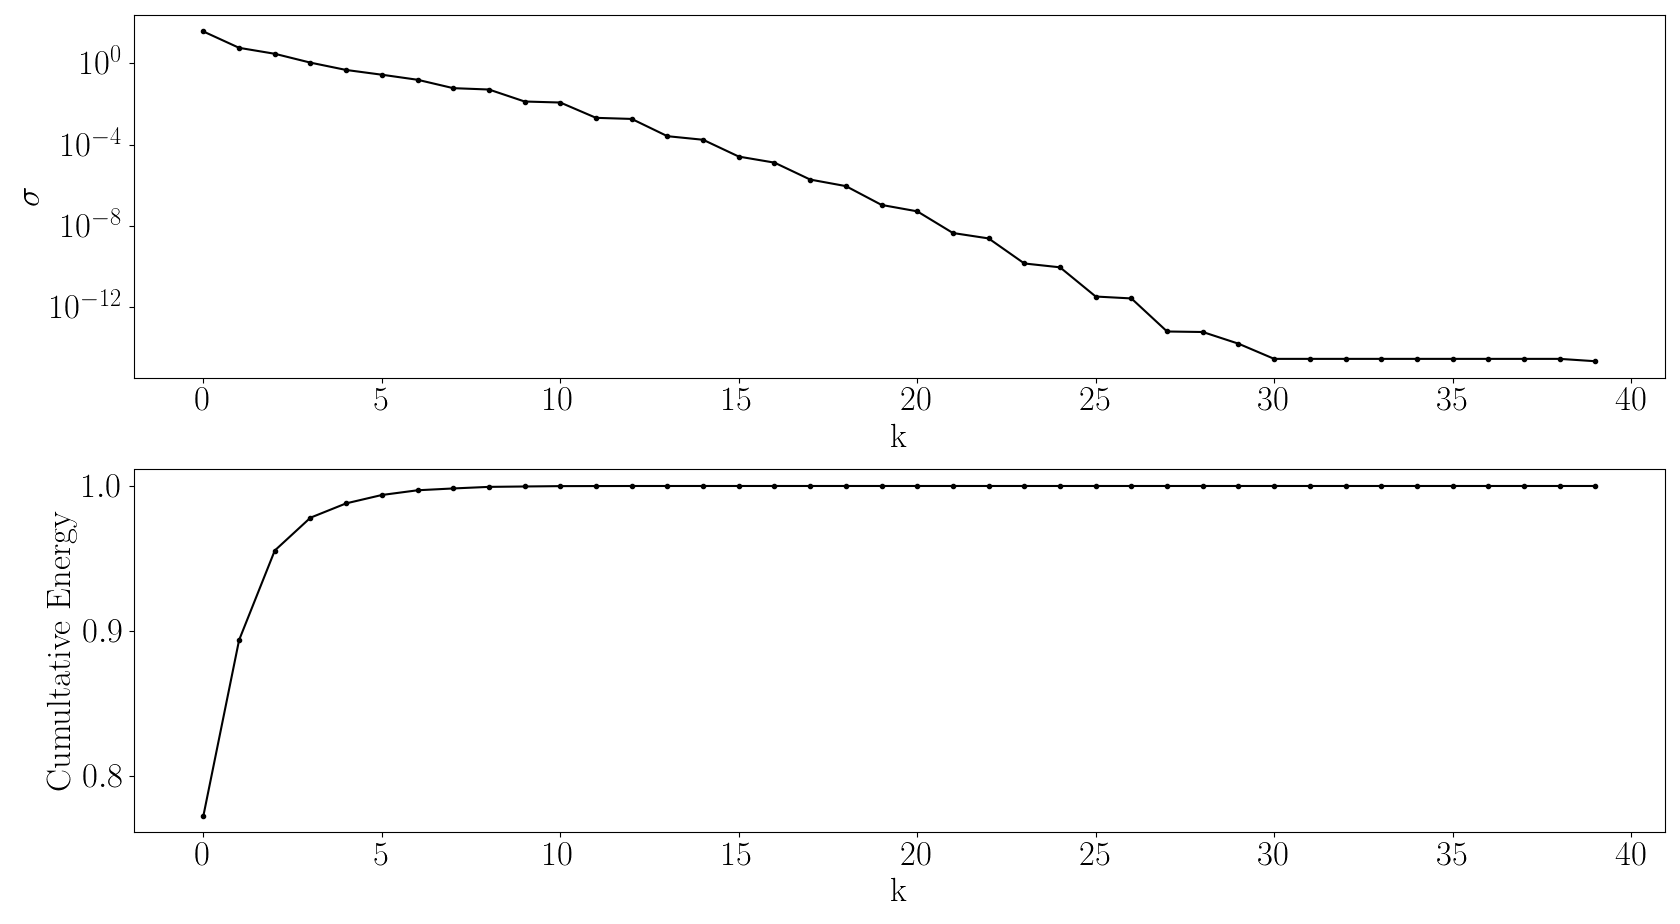
\includegraphics[width=\textwidth]{Figures/Cumultative_Singular_Values_kn001.png}
	\caption{Singular Values (left) and cumultative enrgy (right) over the number of singular values}
	\label{Fig:cumu_sing}
\end{figure}
\subsection{Autoencoders}
The same matrix as in POD is used as input data for the autoencoder:
\[S = \begin{bmatrix}
f(\xi_1,t_1,x_1)&\cdots &f(\xi_n,t_1,x_1) \\
f(\xi_1,t_1,x_2)&\cdots &f(\xi_n,t_1,x_2) \\
f(\xi_1,t_1,x_n)&\cdots &f(\xi_n,t_1,x_n)\\
f(\xi_1,t_2,x_1)&\cdots &f(\xi_n,t_2,x_1)\\
\vdots & \ddots & \vdots\\
f(\xi_1,t_n,x_n)&\cdots &f(\xi_n,t_n,x_n)
\end{bmatrix}\]
During training every 1000 epochs a sample against its prediction was printed in order to link the value of the L1-Loss to a prediction. Using this method a first verification of the model was achieved. Continuing the search for any possible shortage of the models performance, that this method could not cover, eg. samples lying between every 1000 sample, that the model was not able to reconstruct correctly, a second verification process is conducted. 
\section{Results}
\subsection{Evaluation Methods}
In oder to evaluate the proposed dimensionality reduction algorithms, two methods are being introduced. The first one constitutes a qualitative analysis using \cref{Eq:sample_dist} which measures the eucledian distance of every reconstructed sample $\tilde{X}_i$ against it`s corresponding original sample $X$.
\begin{equation}
	|X_i-\tilde{X_i}| = \delta_i \qquad\textrm{with i being the i\textsuperscript{th} sample}
	\label{Eq:sample_dist}
\end{equation}
\begin{equation}
	\sum|\rho_i-\tilde{\rho_i}|=\delta_\rho \qquad\textrm{with i being the i\textsuperscript{th} sample}
	\label{Eq:error_rho}
\end{equation}
As a second quantitative approach a comparison of the density over space in time of the BGK model in \cref{Eq:dense} is utilized. The sum over all euclidian distances from the original samples $\rho_i$ to their reconstruction $\tilde{\rho_i}$ is evaluated in \cref{Eq:error_rho}. 
\begin{equation}
\int_{\Re^3}f(\textbf{x},\xi,t)\colvec{1\\\xi\\\frac{||\xi||^2}{2}}d\xi= \colvec{\rho(\textbf{x},t)\\\rho(\textbf{x},t)U(\textbf{x},t)\\E(\textbf{x},t)}
\label{Eq:dense}
\end{equation}
\subsection{Results}
A quantitative measure shows, that the linear Autoencoder performs slightly better than the POD in the input data.
\begin{center}
\begin{tabular}{ |c|c|c| } 
	\hline
	Algorithm & Density & Samples \\ \hline
	POD & 3.79 & 50.61 \\ 
	AE & 2.52 & 51.21 \\ 
	CAE & cell & cell \\
	\hline
\end{tabular}
\end{center}

\begin{figure}[htb!]
	\centering
	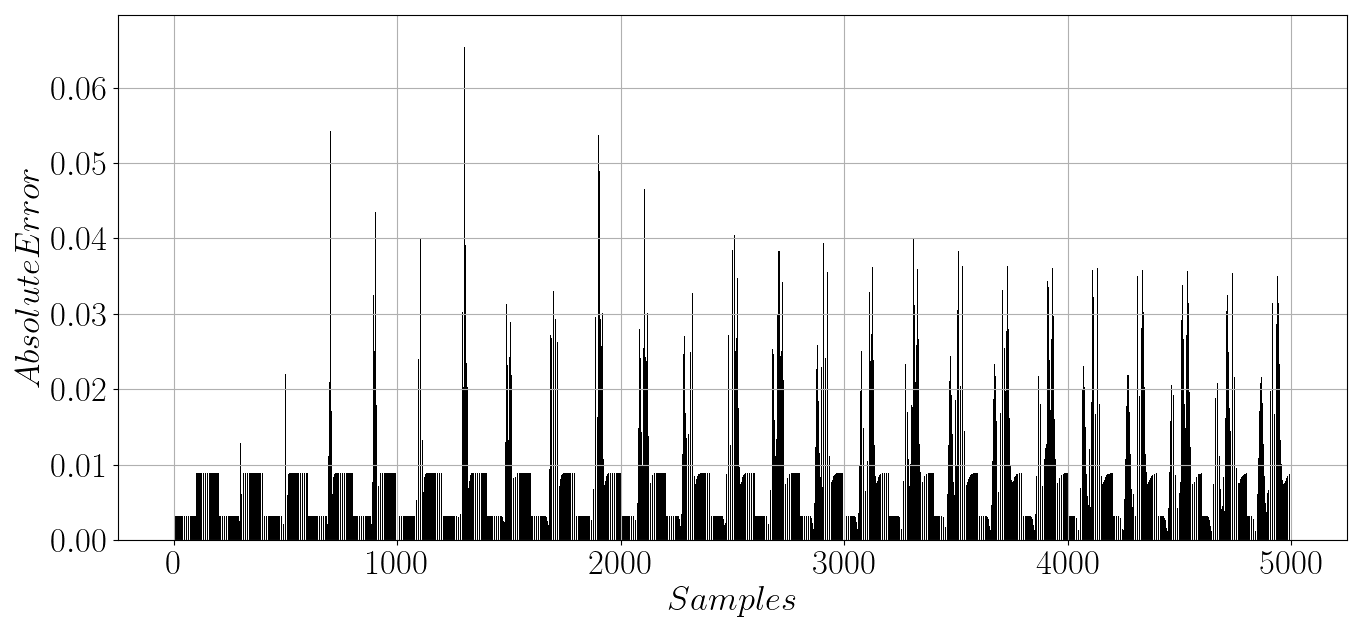
\includegraphics[width=\textwidth]{Figures/Error_samples_SVD.png}
	\caption{Absolute error for every sample in euklidian distance for the POD}
	\label{Fig:Error_samples_svd}
\end{figure}
\begin{figure}[htb!]
	\centering
	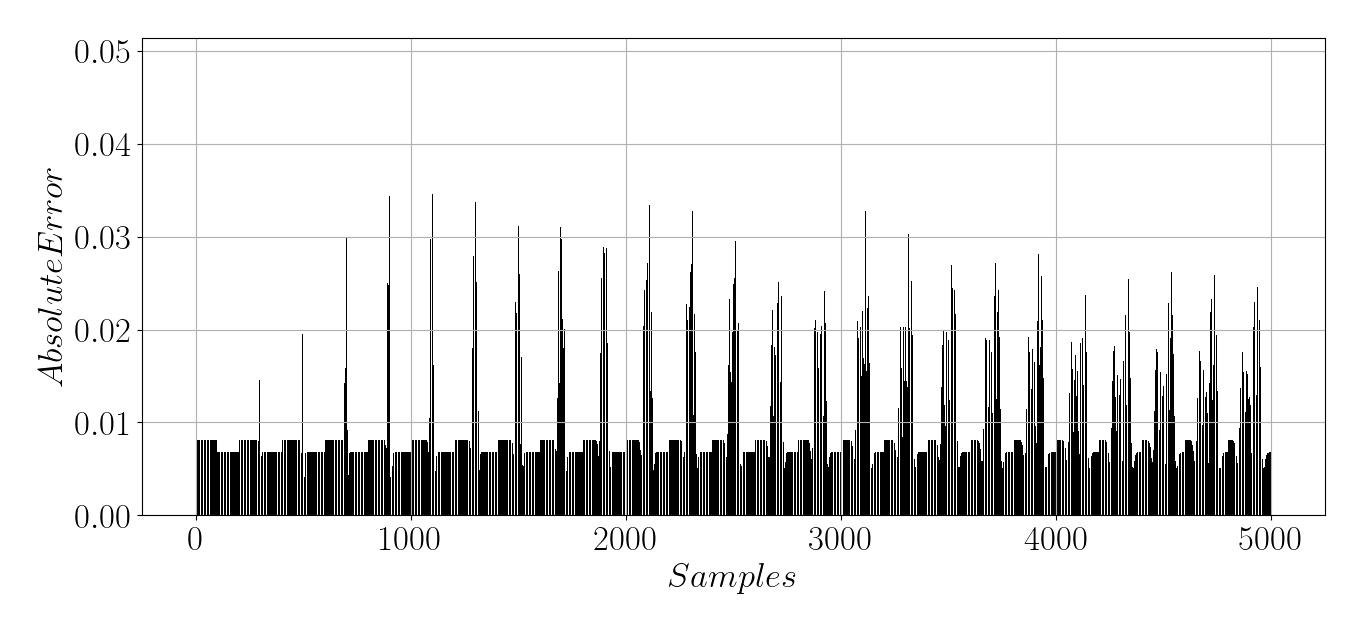
\includegraphics[width=\textwidth]{Figures/Error_samples_v1_1.png}
	\caption{Absolute error for every sample in euklidian distance for the linear autoencoder}
	\label{Fig:error_sample}
\end{figure} 
\begin{figure}[htb!]
	\centering
	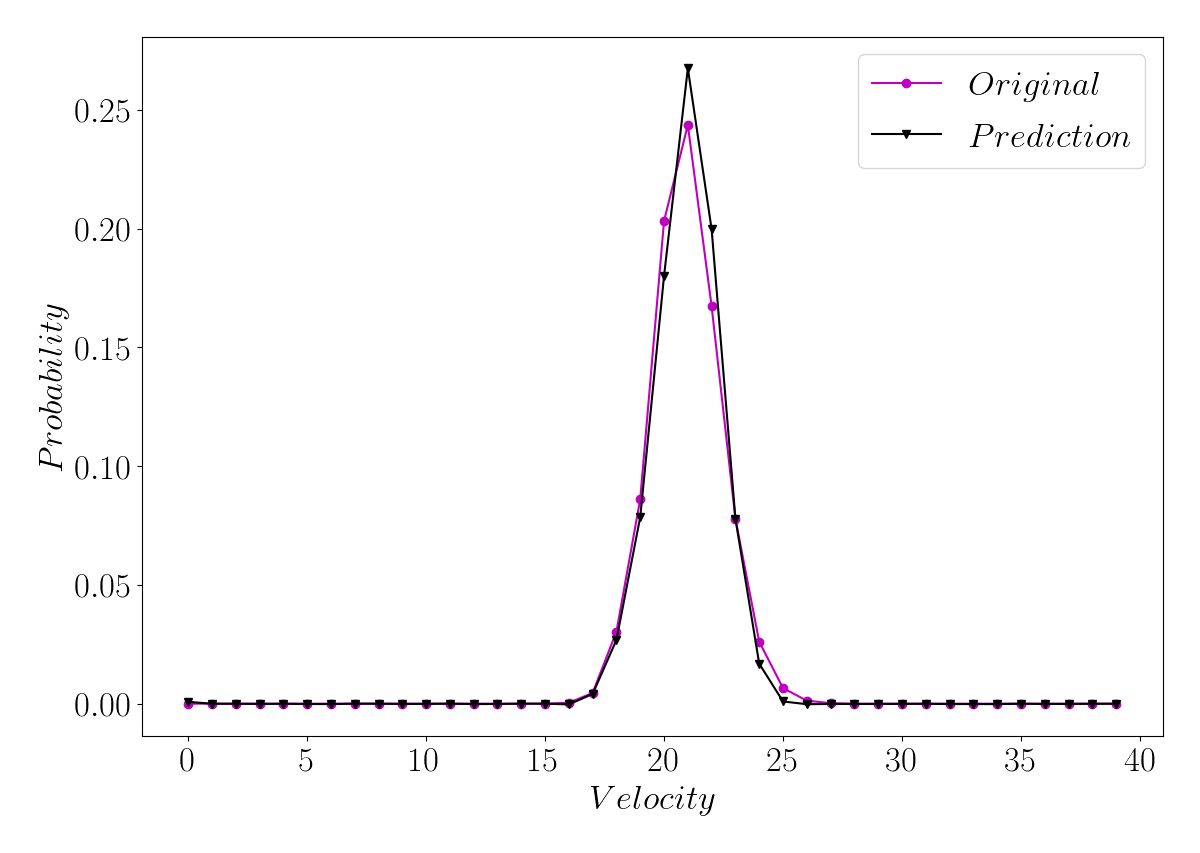
\includegraphics[width=.49\textwidth]{Figures/Sample500_v1_1.png}
	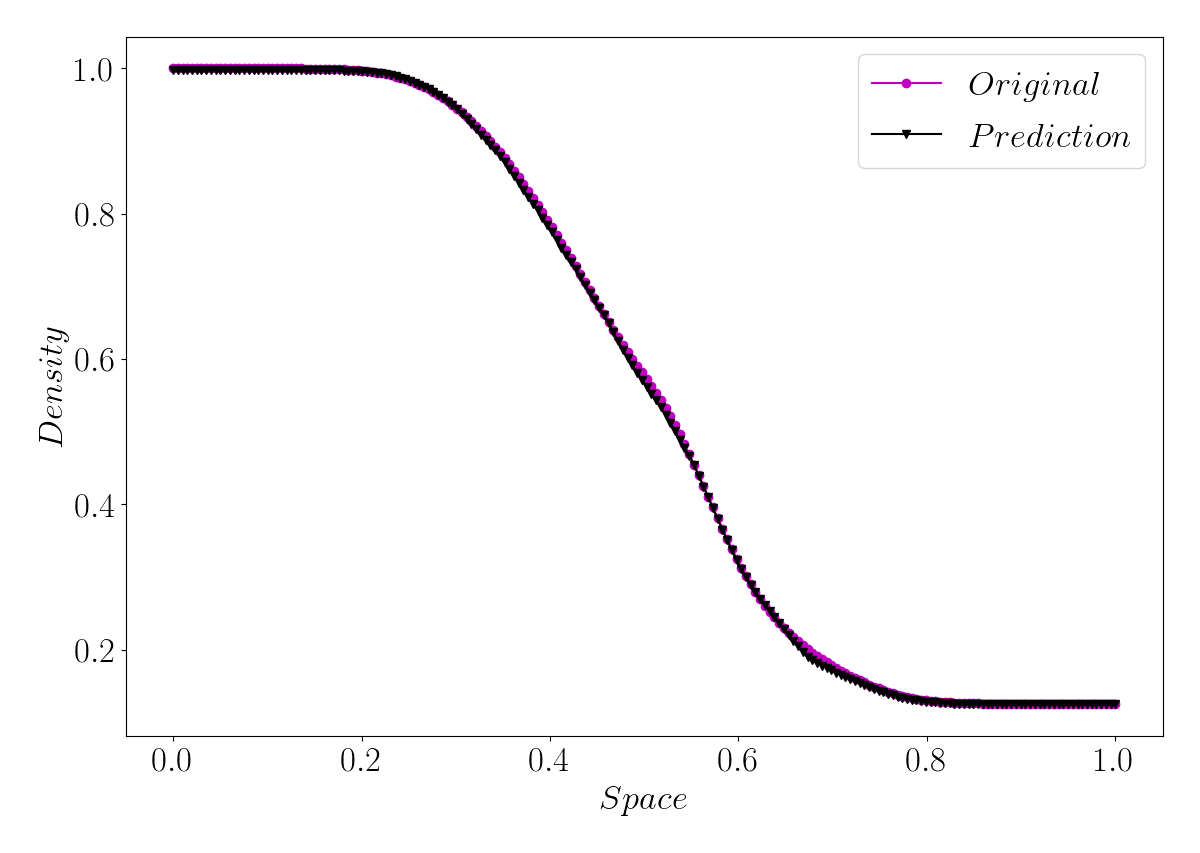
\includegraphics[width=.49\textwidth]{Figures/Density_last_v1_1.png}
	\caption{Error of each sample}
	\label{Fig:Errormore}
\end{figure}
\end{document}